\documentclass{standalone}
\usepackage{tikz}
\usepackage{ifthen}

\begin{document}
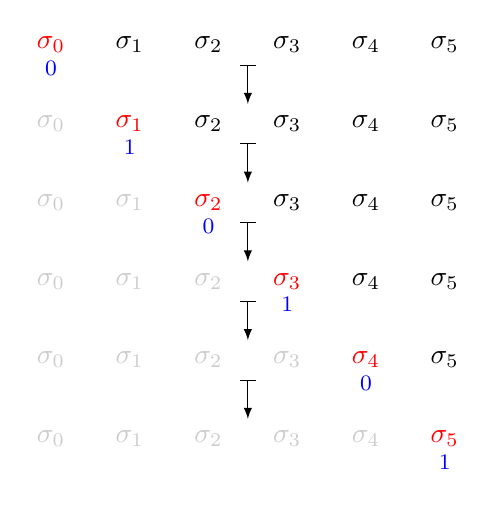
\begin{tikzpicture}
  \pgfmathsetmacro{\nmax}{5}
  \pgfmathsetmacro{\oneless}{\nmax-1}
    \pgfmathsetmacro{\midway}{\nmax/2}

  % Color used to shade the characters we've already read
  \def\viewedcolor{gray!40!white}

  % Function for drawing the diagonal elements properly
  \def\diagelement#1{
    \pgfmathtruncatemacro{\ellabel}{mod(#1, 2)}
    \node[red] () at (#1, -#1) {$\sigma_#1$};
    \node[blue, yshift=-.3cm] () at (#1, -#1) {\footnotesize $\ellabel$};
  }

  \foreach \n in {0,1,...,\nmax}{
    \diagelement{\n}

    \ifthenelse{\n=\nmax}{
      \foreach \k in {0,1, 2, ...,\oneless}{
        \node[\viewedcolor] (s\k\n) at (\k, -\n) {$\sigma_\k$};
      }
    }{
      \pgfmathsetmacro{\ystart}{-\n -.25}
      \pgfmathsetmacro{\yend}{-\n - .75}

      \draw[|-latex] (\midway, \ystart) -- (\midway, \yend);
      \ifthenelse{\n=0}{
        \foreach \k in {1, ...,\nmax}{
          \node (s\k\n) at (\k, -\n) {$\sigma_\k$};
        }
      }{
        \pgfmathtruncatemacro{\nprev}{\n - 1}
        \pgfmathtruncatemacro{\nnext}{\n + 1}

        \foreach \k in {0,...,\nprev}{
          \node[\viewedcolor] (s\k\n) at (\k, -\n) {$\sigma_\k$};
        }

        \foreach \k in {\nnext, ..., 5}{
          \node (s\k\n) at (\k, -\n) {$\sigma_\k$};
        }
      }
    }
  }

\end{tikzpicture}
\end{document}
